\documentclass[a4paper]{article}
\usepackage[utf8]{inputenc}
\usepackage{geometry}
\usepackage{graphicx}

\usepackage[T1]{fontenc}
\usepackage{lmodern}
\usepackage[ngerman]{babel}

\usepackage{float}

\usepackage[colorlinks,
pdfpagelabels,
pdfstartview = FitH,
bookmarksopen = true,
bookmarksnumbered = true,
linkcolor = black,
plainpages = false,
hypertexnames = false,
citecolor = black] {hyperref}

\usepackage[nottoc]{tocbibind}

\title{Projektdokumenation\\Web-basierte Anwendungen\\Verteilte Systeme}
\author{Dennis Meyer\\Dominik Schilling}
\date{\today}

\begin{document}

\maketitle

\newpage

\tableofcontents

\newpage


\section{Einleitung}
Im Rahmen der zweiten Projektphase des Moduls Webbasierte Anwendungen 2: Verteilte Systeme, geht es um die Entwicklung einer Applikation, die sich mit dem Datenaustausch in verteilten Systemen beschäftigt. Innerhalb dieses Systems wird zum einen eine synchrone Kommunikation zwischen Instanzen mit Hilfe des REST Konzeptes realisiert und zum andern ein asynchroner Datenaustausch auf Grundlage von XMPP implementiert. Zur Repräsentation der Funktionalität dient ein selbst entwickelter Client. 

\parskip 12pt
\parindent 0pt
Folgendes Dokument erfasst die einzelnen Entwicklungsschritte. Von der anfänglichen Konzeptidee inklusive Konzeption der benötigten XML Schematas, über die Implementierung des RESTful Webservices und XMPP Client, bis hin zur Umsetzung des grafischen User Interfaces. Dabei werden, neben den finalen Ergebnissen, auch getroffene Abwägungen, Entwicklungen und Entscheidung hinsichtlich der Umsetzung dargestellt und erläutert. 
Zuletzt folgt eine Projektreflektion, anhand derer Erfahrungen für weitere Projekte mitgenommen werden sollen.


\section{Konzept}
Zu Beginn des Projektes ging es um das Finden eines geeigneten Anwendungsfall aus der Realität. Für diesen sollte das geforderte System, eine sinnvolle Ergänzung für mögliche Anwender darstellen.
Zum einen muss die Möglichkeit bestehen, Informationen direkt auszutauschen und zum anderen sollte eine Art Benachrichtigungssystem existieren, bei denen die Interessenten nur beim Eintreten bestimmter Ereignisse informiert werden müssen.
Nach Überlegung fiel dabei die Wahl auf das Thema Film und Fernsehen und wurde im Spezielleren auf Serien eingegrenzt. Sinnvoll erscheint eine Umsetzung dieses Thema aufgrund der regelmäßigen Ausstrahlung von Folgen einer bestimmten Serie.
Während man für einen Film lediglich einmal die Ausstrahlungszeit in Erfahrung bringen muss, würde sich dieser Schritt bei Serieninteressierten Woche für Woche wiederholen. Dazu kommen kurzfristige Änderung im Fernsehkalender, die im unpassenden Fall dazu führen, dass eventuell Folgen verpasst werden. Schaut jemand nicht nur eine Serie, sondern hat eine Art festen Wochenplan, so kann hierbei auch der Überblick darüber verloren gehen, welche Folge man eigentlich zuletzt gesehen hat oder wie die Serie hieß, die einem neuliche empfohlen wurde. 

\parskip 12pt
\parindent 0pt
Mit dieser grundlegenden Überlegung ging es an das Konzipieren des Funktionsumfangs der Applikation unter dem Projekttitel \textbf{Serientracker}.
Die Idee ist, dass Serieninteressierte\footnote[1]{Innerhalb des Kontext wird für den Benutzertyp des Anwenders/Nutzers auch diese Bezeichnung verwendet werden, da diese Personengruppe in ihrer Funktion die Benutzer des Systems darstellen werden.} die Möglichkeit besitzen bestimmte Serien zu favorisieren und Meldungen zu gewissen Themen abonnieren können. Er soll Zugriff auf einen Pool von Serien bekommen, die auf einem Server gespeichert und verwaltet werden. Der Benutzer erhält dann zu seinen Lieblingsserien Benachrichtigungen, sobald eine Episode dieser Serie im TV ausgestrahlt wird. Wenn vorher noch das Genre Comedy abonniert wurde, so erhält er zudem noch eine Benachrichtigung, welche Serien dieses Typs aktuell so laufen.
Außerdem soll die Möglichkeit bestehen eine Episode zu bewerten und als gesehen/ungesehen zu markieren. Diese Verwaltung findet innherhalb von privat angelegten Listen statt, die neben der klassischen Seen/Unseen Form auch als Watchlist oder ähnliches definiert werden kann.

\newpage
Die \textbf{Server-Anwendung} soll die Nutzer über die TV-Austrahlung einer Episode zu einem Zeitraum informieren, die sich der Benutzer selbst definiert hat. Er kann demnach entscheiden, ob ihm eine Benachrichtigung für die ganze Woche genügt, ob er jeden Morgen über den aktuellen Tag informiert werden möchte oder eine Meldung 5 Minuten vor Sendestart ausreicht, da er planmäßig zu Hause sein wird.

\parskip 12pt
\parindent 0pt
Ein \textbf{Content-Admin} soll erweiterte Rechte bekommen, um die Content-Verwaltung zu übernehmen. Die Anwendung soll das Anlegen, Bearbeiten und Löschen von Serien bzw Episoden ermöglichen. Zudem ist somit das Korrigieren von Fehlern möglich, die von Usern eingeschickt werden oder die aufgrund von Planänderungen anfallen.

Als möglicher Zusatz ist eine Einbindung von Freunden geplant. Nutzer sollen sich gegenseitig hinzufügen/abonnieren können um sich gegenseitig zu benachrichtigen. Zum Beispiel in Form von \textit{Freund X schaut gerade Y}, \textit{Freund Z hat Serie/Episode mit 8,0 bewertet} oder \textit{Freund Y empfiehlt dir Serie W}. Ob dieser Ansatz innerhalb des Projektes realisiert wird, hängt vom vorranschreiten der Umsetzung  und der damit einhergehenden Abwägung für das eigentlich Ziel des Projektes ab.
\subsection{Umsetzung}
Zuvor genannte Funktionen würden, für einen Informationsaustausch zwischen Server und Anwendung, hinsichtlich folgender Einstufung der Datenübertragung umgesetzt werden.

\subsubsection{Synchrone Datenübertragung}

Zum einen hat der Anwender direkt die Möglichkeit auf Informationen in Form von Daten zuzugreifen und diese zu Manipulieren.

\begin{itemize}
\item
Serien-Interessierte
	\begin{itemize}
	\item
    Markieren von Episoden
    	\begin{itemize}
    	\item
     	Gesehen/Nicht gesehen
     	\end{itemize}
    \item
    Bewertung einer Episode
      	\begin{itemize}
      	\item
        Kommentar
        \item
        Bewertung in Zahlen
        \end{itemize}
     \item
     Fehlermeldung
     	\begin{itemize}
     	\item
        geänderte Sendezeit, fehlerhaftes Datum
        \end{itemize}
     \item
     Listen
     	\begin{itemize}
     	\item
    	Ausgabe (Un)Watched
    	\item
     	Ausgabe vorhandene Serien
     	\item
     	Ausgabe Follower/Following (?)
     	\end{itemize}
     \item
     Favorisierung
   	  	\begin{itemize}
   	  	\item
   	  	Anlegen
   	  	\item
   	  	Löschen
   	  	\item
   	  	Bearbeiten
   	  		\begin{itemize}
   	  		\item
   	  	    Zeitpunkt der Benachrichtigung
   	  	    \end{itemize}
		\end{itemize}
	\end{itemize}
	\item
	Content-Admin
		\begin{itemize}
		\item
		Verwaltung der Episoden
			\begin{itemize}
			\item
			Anlegen
			\item
			Löschen
			\item
			Bearbeiten
			\end{itemize}
		\end{itemize}
\end{itemize}


\subsubsection{Asynchrone Datenübertragung}

Ein weiterer Aspekt ist das Anfordern von Informationen, wobei die entsprechenden Informationen von Seiten des Servers von Bedingungen abhängig gesendet werden, was auch mehrfach geschehen kann.

\begin{itemize}
\item
Serien-Interessierte
	\begin{itemize}
	\item
    Benachrichtung bei TV-Austrahlung
    \item
    Freunde mit gleicher Favorisierung bei Serienstart mit Check-in benachrichtigen (?)
	    \begin{itemize}
	    \item
         Freund X schaut auch W
         \end{itemize}
    Empfehlung einer Serie von Freund(e) anzeigen (?)
    \end{itemize}
\item
Content-Admin
	\begin{itemize}
	\item
    Benachrichtung bei Fehlermeldung durch User
    \end{itemize}
\end{itemize}

\subsubsection{Kommunikationsabläufe}
Im Rahmen des Konzeptes wurden zwischen dem Server und dem User (hier repräsentativ für die Anforderung seitens der Anwendung) folgende Kommunikationsabläufe identifiziert.
Die synchronen Interaktionen werden vom User iniziiert und greifen auf die beim Server abgelegten Datensätze zu. Dabei hat jeder User die Möglichkeit eine einfache Anzeige der Daten anzufordern oder eine Serie den Favoriten hinzuzufügen. User mit erweiterten Adminrechten wird hierbei auch die Manipulation der Daten gewährleistet, um eine Verwaltung zu ermöglichen. Die entsprechende Repräsentation der Information wird vom Server wieder an den User zurück gegeben. 
Diese Ansätze werden über einen RESTful Webservice umgesetzt und mit entsprechenden GET, POST, PUT und DELETE Methoden realisiert.\footnote[2]{Dazu mehr in...}

\begin{figure}[H]
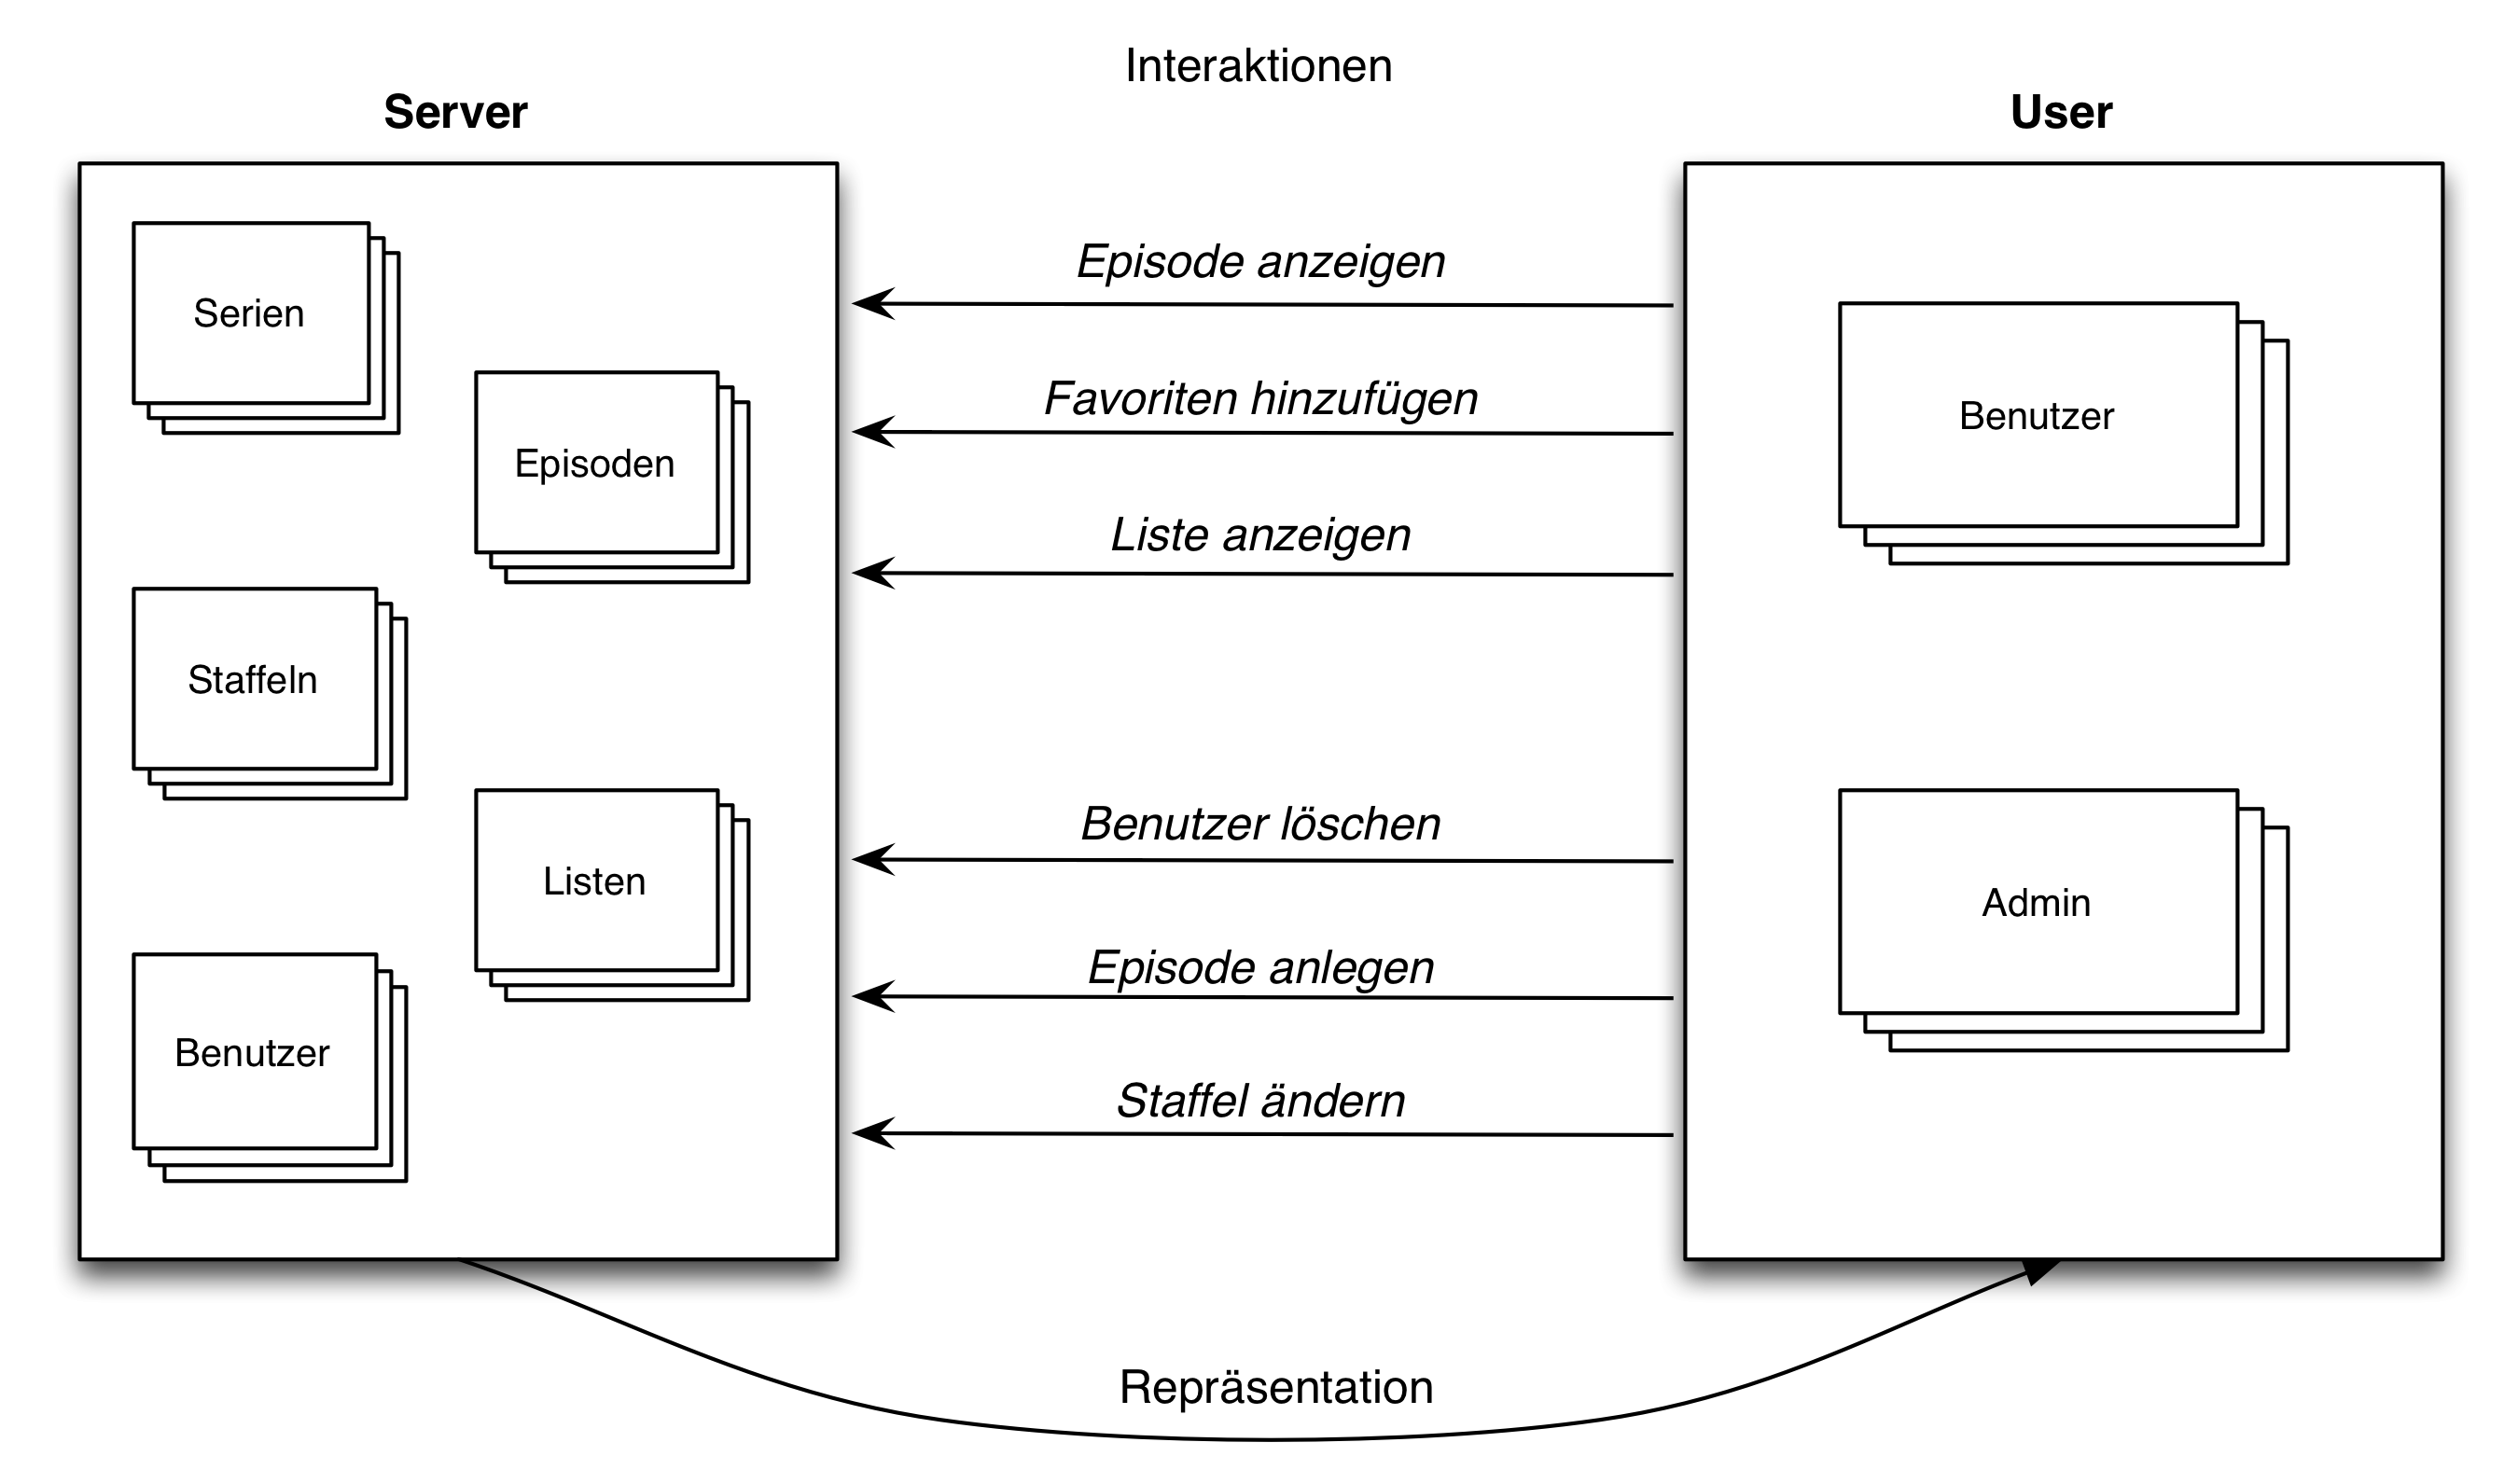
\includegraphics[width=1\textwidth]{images/kommunikationsablaeufe.png}
\caption{Synchrone Kommunikationsabläufe}
\label{kommunikationsablaeufe}
\end{figure}

Die Asynchronen Kommunikationsabläufe liefern Informationen bei bestimmten Events vom Server an die entsprechenden User als Empfänger. Dieser Ansatz wird mit Hilfe von XMPP realisiert werden und ist im Kapitel X.X genauer dargelegt. 

\begin{figure}[H]
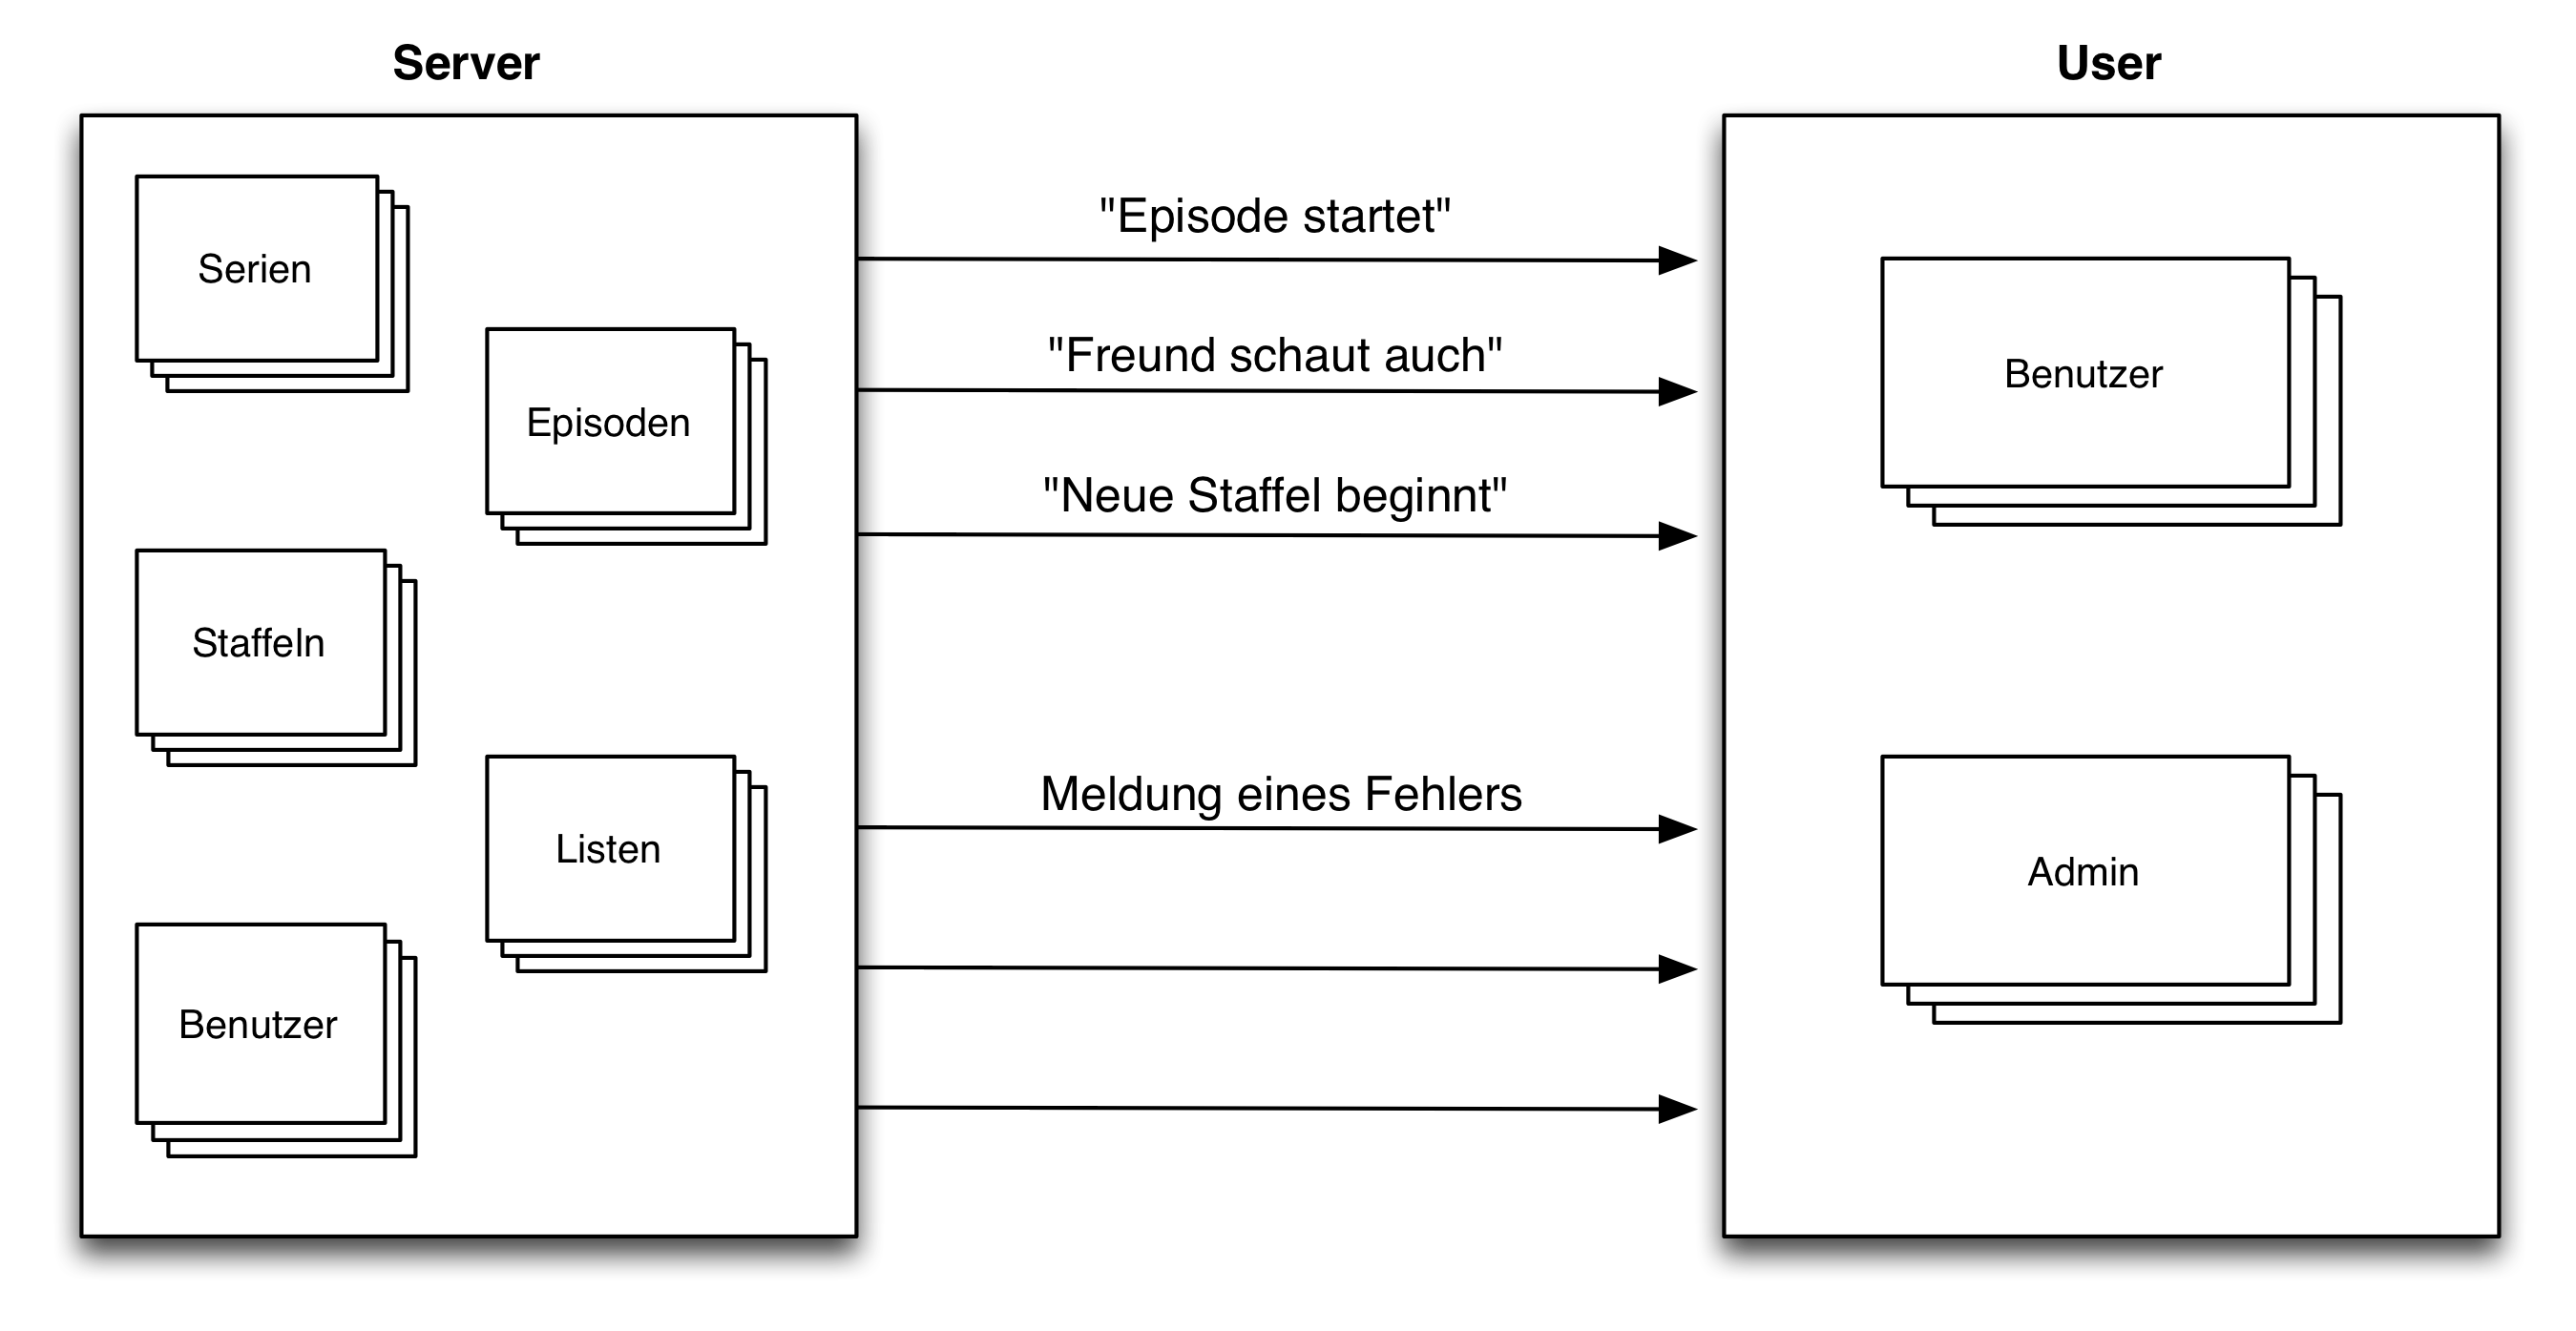
\includegraphics[width=1\textwidth]{images/kommunikationsablaeufeAsynchron.png}
\caption{Asynchrone Kommunikationsabläufe}
\label{kommunikationsablaeufeAsynchron}
\end{figure}


\newpage

\section{Entwicklung des Projektes}

\subsection{Projektbezogenes XML Schema / Schemata}
\subsubsection{Vorüberlegungen}
Der erste Meilenstein befasst sich mit der Repräsentation von Daten in XML.

Damit bei der Verwendung der XML Dateien bei der späteren Verarbeitung mit JAXB keine Probleme auftreten,
ist es notwendig eine Validierung der Dateien durch Definition zugehöriger XML Schemas durchzuführen.
Vorteil bei der Verwendung eines Schemas ist, neben der Kontrolle auf Wohlgeformtheit und der Verwendung
definierter Datentypen und Strukturen, auch das festlegen von Restriktionen.

Hinsichtlich des zugrunde liegenden Konzeptes und den benötigten Informationen, gibt es viele Elemente
innerhalb der Dateien, die nur mit Strings realisiert werden können. Das Problem bei freier Definition
besteht darin, dass die Datensätze sehr fehleranfällig sind, wenn es um die Benutzung durch Menschen geht.
Rechtschreibfehler beim Namen des Landes, des Fernsehsenders oder des Genres, würden für den Leser bzw.
Interessenten der Anwendung noch kein Problem darstellen, da er vermutlich deuten könnte was gemeint ist.
Informationstechnisch ist es aber von Vorteil, die Datensätze möglichst konsistent und reichhaltig anzulegen.

Das System des Serientrackers beruht darauf, die Verwaltung von Serien anhand von Listen und Tags wie
Gesehen, Ungesehen zu ermöglichen. Wie bereits in der Besprechung der Umsetzung erwähnt, wird anhand
dieser Informationen auch die Asynchrone Datenübertragung realisiert.
Das Abonnieren von Informationen zu laufenden Serien des Genre Krimi, greift bei Benachrichtigung auf
Datensätze zu, die diesem Elementwert unter dieser eindeutigen Zeichenfolge zugeordnet sind. Formulierungsfehler
wie Krimie oder Crime, führen dementsprechend zu Komplikationen, weil sie die Konsistent der Informationssätze beschädigen.

Die Auseinandersetzung führte zu dem Ergebnis, dass folgende Objekttypen innerhalb des Serientrackers von interesse sind und wiederkehrende Elemente darstellen:

Serie \\
Eines der wichtigsten Elemente, dass alle Informationen beinhaltet, die für den Benutzer von bedeutung sind, ist die Serie. 
Eine Serie besitzt allgemeine Informationen wie Name, eine Beschreibung, der Sender indem sie ausgestrahlt wird oder das Produktionsland.
Im realen Kontext wird eine Serie zudem in Staffeln ausgestrahlt, die jeweils eine bestimmte Anzahl von Episoden enthalten.

Staffel \\
Bestandteil einer Serie, von der es im Laufe der Jahre immer neue Objekte gibt und die nach einer gewissen Anzahl an Episoden als abgeschlossen gelten.

Episode \\
Ein Kernelement des Systems, dass ein wichtigen Typ für die asynchrone Kommunikation darstellt. Durch das Abonnieren von Genres oder Serien, wird die Benachrichtigung in Bezug auf eine einzelne Episode ausgelöst, die sich durch ihr jeweiliges Austrahlungsdatum und -zeitpunkt kennzeichnet. 
Zudem kann der Inhalt der Episode von Interesse sein.

User \\
Neben den Serieninformation, gibt es die Anwender des Serientrackers, die sich anmelden und durch Listen die Dienste des Serientrackers abonnieren.
Allgemein werden hierbei personenbezogene Daten wie Username und echter Name erwartet, so wie Zusatzinformationen, die für andere Benutzer von Interesse sein könnten und die Person hinter dem Profil genauer beschreiben. Beispiele wären das Alter, ein Profilbild, Wohnort oder eine kurze Beschreibung.

Liste \\


Als zusätzlicher Typ, der jedoch erst in der asynchronen Kommunikation verwendung finden wird, wurde die Message, also eine bestimmte Art von Nachricht identifiziert.

Für diese Obertypen gilt es ein valides XML Schema zu definieren, wobei während der Entwicklung verschiedene Aspekte betrachtet werden müssen.  

\newpage

\subsubsection{Datentypen}
Bei der Definition eines XML Schemas, sollte neben der enstprechenden Datensatzstruktur auch festgelegt werden, durch welche Datentyp die einzelnen Informationen repräsentiert werden sollen.

\newpage

\subsubsection{Restriktionen}
Um die eingegeben Daten semantisch sinnvoll zu halten, wurde für einige Elemente und Attribute Bedindungen hinzugefügt, die im jeweiligen Zusammenhang sinnvoll erscheinen. 

\begin{table}[H]
\caption{Restriktionen des User Schemas}
\centering

\begin{tabular}{l l l}
\\ [-0.5ex]

\hline\hline
\\ [-0.5ex]
Element/Attirbute & Restriktion & Begründung
\\ [1.5ex]
\hline
\\ [-0.5ex]
Username & Stringlänge 2 < und < 30 & sinnvolle Namenlänge,\\[1ex]
&& verhindert Text \\[3ex]

Lastname & Stringlänge 1 < und < 40 & gängige Nachnamenlänge, \\[1ex]
&&eventuell Doppelnamen,\\[1ex]
&&verhindert Text \\[3ex]

Firstname & Stringlänge 1 < und < 50 & gängige Vornamenlänge, \\[1ex]
&&Mehrfachnahmen \\[3ex]

Gender & Auswahl zwischen Male und Female & logische Auswahl, \\[1ex]
&&Vorgabe verhindert Schreibfehler\\[3ex]


Age & älter als 13 und jünger als 121 & Mindestalter zur Nutzung, \\[1ex]
&&logische Obergrenze \\[3ex]

Location & Stringlänge < 40 & Stadtname, Land etc. \\[1ex]
&&Eingabe ist keine Adresse\\[1ex]
&&und lässt sich in Kürze ausdrücken\\[3ex]

About & Stringlänge < 200 & optionale Kurzbeschreibung,\\[1ex]
&&nach oben begrenzt, \\[1ex]
&&zu viele Informationen nicht \\[1ex]
&&unbedingt von Interesse  \\[3ex]

Admin & Boolean ob True or False & Rechtevergabe nach Status,\\[1ex] 
&&Auswahl nur in 2 Zuständen möglich\\[2ex]

\hline
\end{tabular}
\label{tab:restriktionenderxsd}
\end{table}


\begin{table}[H]
\caption{Restriktionen des Serie Schemas}


\begin{tabular}{l l l}
\\ [-0.5ex]

\hline\hline
\\ [-0.5ex]
Element/Attirbute & Restriktion & Begründung
\\ [1.5ex]
\hline
\\ [-0.5ex]
Year & Jahreszahl 1900 < und < 2015 & Jahreszeiten außerhalb\\[1ex]
&&unrelevant \\[3ex]

Country & Auswahlmöglichkeit Ländern & Eingabefehler verhindern\\[3ex]
Episoderuntime & Auswahl zwischen gängigen Episodenlängen& Serie hat feste Episodenlänge\\[3ex]
Network & Auswahl bekannter Sender & unrelevante Sender entfallen,\\[3ex]
&&Eingabefehler verhindern\\[3ex]

Airday & Auswahl des Tagnamen & Eingabefehler verhindern\\[3ex]
Genre & Auswahl definierter Genres & einheitliche Schreibweise,\\[1ex]
&&Eingabefehler verhindern,\\[1ex]
&& sinnvolle Genre\\[2ex]

\hline
\end{tabular}
\label{tab:restriktionenderxsd}
\end{table}




\begin{table}[H]
\caption{Weitere Restriktionen}


\begin{tabular}{l l l}
\\ [-0.5ex]

\hline\hline
\\ [-0.5ex]
Element/Attirbute & Restriktion & Begründung
\\ [1.5ex]
\hline
\\ [-0.5ex]
Overview (global) & Stringlänge 10 < und < 500 & allgemeinen Informationen,\\[1ex]
&&kurze Inhaltsangabe\\[3ex]
Title (global) & Stringlänge 1 < und < 80 & gängige Titellänge\\[3ex]
Name (list) & Stringlänge 2 < und < 80 & treffende Bezeichnung,\\[1ex] 
&&Name keine Beschreibung \\[3ex] 
Public (list) & Boolean True und False & feste Zustände \\[3ex] 
Episodenumber (episode) & Anzahl < 26 & sinnvolle maximale Episodenanzahl\\[3ex] 
Seasonnumber (seasons) & Anzahl < 41 & sinnvolle Begrenzung, \\[1ex]
&&Freiraum für Langzeitserien \\[2ex] 

\hline
\end{tabular}
\label{tab:restriktionenderxsd}
\end{table}

Neben diesen Restriktionen einzelner Elemente bezogen auf ihre Werte, bestehen auch Genehmigungen bei Containerelementen, hinsichtlich der Häufigkeit für vorkommende Elemente. TODO

Weiterer Aspekt der Definition der Attribute war das festlegen des Benutzungstyp. Da wir Elemente wie Episode haben, die als eigener Typ definiert werden können, aber in einem bestimmten Kontext stehen, werden hierbei Attribute verwendet um die genaue zuordnung zu gewährleisten. Für diese charakterisiernden Attribute, die für spätere Abfragen notwendig, wurde dieses Attribute mit dem Usecase required versehen. Eine Episode erfordert demnach eine genaue serieID, seasonID und episodeID, da sie genannten Nutzen aufweisen. Weiterhin lässt sich einer List eine jeweilige globale listID, eine userID des Verwalters und die Rechtevergabe public zuordnen, da auch diese Informationen als notwendig angesehen werden und im späteren Kontext im Zusammenhang des Serientrackers von Bedeutung sein können. 

\newpage
\subsubsection{Umsetzung}

Nach der theoretischen Planung findet die Realisierung der XML Schemas statt.
Dabei wurde für jeden der zuvor identifizierten Obertypen ein eigenes Schema definiert. Die Aufteilung der einzelnen Typen auf ein seperates Schema, fand mit den Gedanken statt, die Struktur der Daten möglichst einfach und lesbar zu halten. Eine Serie die mehrere Staffeln enthält, die wiederrum jeweils eine Menge von Episoden auffassen, würde ein sehr komplexes Elemente definieren, dass bei der späteren Verarbeitung zu Komplikationen führen kann.

Da die Daten einer Episode, inhaltlich jedoch weiterhin davon abhängen, von welcher Serie diese ist und in welcher Staffel sie vorkam, wird eine Referenzierung mit Hilfe von global eindeutigen IDs eingeführt. Jede Serie, User, Staffel, Episode und Liste wird mit einer einzigartigen Folge von Zeichen beschrieben, über diese es möglich ist auf gewünschte Informationen zuzugreifen und entsprechende Elemente auszulesen.

Eine Episode bekommt damit eine eindeutige episodenID zugeordnet, erhält zudem aber die Referenz der serienID und seasonID als Attribute, um Verweise und Zuordnungen zu realisieren. Da sich jedes Objekt demnach durch eine Kennung repräsentiert, reicht bei anlegen von Listen und Containern ein einfacher Verweis auf entsprechendes Element, wodurch Datenredundanz bei Schemen verhindert wird, die inhaltlich voneinander abhängen.

Um die Struktur des gesamten Serien Elements zu ermöglichen und vorhandene IDs global nutzen zu können, wird jedes Schema über eine Masterdatei in die einzelnen XML Schemas inkludiert, um bereits definierte Elemente und Attribute wiederverwendbar zu machen und die Datenmenge zu reduzieren.


Ein weiterer Gruppe von Elementen, die bei der Entwicklung eine wichtige Rollen spielen sind die Containerelemente. Da jede Entität eines Typs angelegt werden muss, wurde für jeden verwendeten Typ User, Serie, Season, Episode, List, eine eigene Liste angelegt, die jedes Elemente ihres speziellen Typen aufnehmen und als Containerklasse dienen.


\newpage

\subsection{Ressourcen und die Semantik der HTTP-Operationen}
\subsubsection{Ressourcen}

Als Vorbereitung für die Umsetzung der synchronen Kommunikationsvorgänge, steht die theoretische Auseinandersetzung mit REST im Mittelpunkt.
Der erste Schwerpunkt dabei ist die Identifizierung vorhanderer Ressourcen des Serientrackers. Bereits beim Konzipieren der XML Schemas mit beispielhaften XML Datensätzen, musste überlegt werden, für welche Elemente es möglich ist Enitäten der realen Welt zu ermitteln.

Bei einer Ressource geht es, ähnlich wie bei XML Dateien, nicht darum wie die darin enthalten Informationen im letztendlichen Kontext repräsentiert werden, sondern welche Informationen diese enthalten. Entsprechende Objekte der Außenwelt werden beschrieben und wie die Wurzelelemente bei XML, stellen sie einen bestimmten Objekttyp dar. Eine identifizierte Ressource, ist eine Schnittstelle zur Außenwelt und sollte daher dem Kontext entsprechend gut durchdacht werden.
Die Auseinandersetzung im Rahmen mit den XML Schemas lieferte dabei einen Überblick über vorhandene Primärressourcen. Dabei handelt es sich um die Oberklassen der vorhandenen Objekttypen Serie und User.

Desweiteren ist es möglich vorhandene Subressourcen zu identifizieren, die sich dadurch auszeichnen, dass sie selbst Bestandteil einer Ressource sind.
Aufgrund der komplexen Struktur einer Serie, die neben den allgemeinen Informationen noch die Informationen zu mehreren Staffeln und entsprechenden Episoden enthalten, wurde früh die systematische Aufteilung festgelegt.
Da es auch innerhalb der Anwendung von Interesse sein kann, eine einfache Repräsentation der Staffelübersicht oder der Episodenübericht einer Staffel zu ermöglichen, bietet es sich gerade bei diesen Typen an, diese Objekte als eigene Ressource zu designen. Dazu kommt, dass eine Episode zum Beispiel im Kontext einer Serie am meisten Sinn macht, durchaus aber auch für sich existieren kann.

Zur Ordnung der einzelnen Elemente, gibt es entsprechende Listenressourcen wie Series, Seasons, Users und Episodes, welche alle Elemente des zugehörigen Typs aufnehmen und sammeln.

Ein Kernelement der Anwendung, wird das Benachrichtigen der Benutzer über bestimmte Eregnisse sein, die sich durch Abonnements in Form von Listen verwalten lassen. Gerade bei einer möglichen Kategorisierung wie Serie nach dem Genre Drama, wäre es durchaus interessant gewesen Listenressourcen mit entsprechenden Filtern zu definieren. Aufgrund der Vielzahl von Kategorisierungsmöglichkeit, wird dieser Schritt aber nicht über einzelne Ressourcen stattfinden, sondern über die Anwendung mit Verweisen innherhalb der Listen geregelt.

\newpage

Die Auseinandersetzung führte zu folgenden Ressourcen, wobei die angegeben URI nur den charakteristischen Abschnitt wiederspiegelt.
Da für die Umsetzung an sich, die URI eher als eine ID in Form von Zeichen steht und für die letzendliche Auswertung nicht unbedingt notwendig ist, wird auf eine Darstellung in Form mit Schema und Pfadangabe in der Übersicht verzichtet.


\begin{table}[H]
\caption{Ressourcen des Serientrackers}

\centering
\begin{tabular}{l l l}
\\ [-0.5ex]

\hline\hline
\\ [-0.5ex]
Ressource & URI & Methode
\\ [1.5ex]
\hline
\\ [-0.5ex]
Liste aller Serien & /series/ & GET, POST \\[1ex]
Einzelne Serie & /series/\{id\} & GET, PUT, DELETE\\[1ex]
Liste aller Staffeln & /seasons/ & GET, POST \\[1ex]
Einzelne Staffel & /seasons/\{id\} & GET, PUT, DELETE\\[1ex]
Liste aller Episoden & /episodes/ & GET, POST \\[1ex]
Einzelne Episode & /episodes/\{id\} & GET, PUT, DELETE\\[1ex]
Liste aller User & /users/ & GET, POST \\[1ex]
Einzelne User & /users/\{id\} & GET, PUT, DELETE\\[1ex]
Liste aller Listen & /lists/ & GET, POST\\[1ex]
Liste eines Users & /lists/\{id\} & GET, PUT, DELETE\\[1ex]
\hline
\end{tabular}
\label{tab:ressourcendesserientrackers}
\end{table}

Jedes Element, dass für die synchrone Kommunikation von Interesse ist, besitzt eine Ressource auf ein einzelnes Element und die Gesamtheit einer Liste. Bei den URI wird der Zugriff über entsprechende ID's auf die Liste deutlich und es zeigt sich eine Folge der einfachen Ressourcen. Durch die Konzipierung der Untertypen Staffel und Episode als einzelne Ressource, wird eine komplexe Hierachie verhindert, die in Form von /series/\{id\}/seasons/\{id\}/episodes/\{id\} dennoch realisierbar gewesen wäre.


\subsubsection{Parameter}

Die Repräsentation einer spezifischen Ressource wurde im vorherigen Abschnitt mittels \textbf{Path-Parameter} realisiert, das heißt, der Parameter ID war Teil der eigentlichen URI.\\
Als Alternative können allerdings auch sogenannte \textbf{Query-Parameter} zum Einsatz kommen. Diese eignen sich meistens um Ressourcen noch weiter zu verfeinern und sind in der Regel optional.

Exemplarisch könnte ein Query-Parameter in diesem Projekt bei der Ressource Users zum Einsatz kommen, um nur die Benutzer der Gruppe Admin zu repräsentieren: \textsf{/users/?group=admins}. Aber auch bei einem Zugriff auf eine einzelnen Episode einer Staffel einer Serie können Query-Parameter genutzt werden, Beispiel: \textsf{/episodes/?serie\_id=1\&season\_id=2}. Jedoch wären die Parameter an dieser Stelle obligatorisch.

Als Alternative zu den beiden Varianten bietet sich noch der \textbf{HTTP-Header} des Clienten an. Da diese Art von Parameterübertragung eher untypisch ist, wird an dieser Stelle nicht weiter drauf eingegangen.

\subsubsection{Semantik der HTTP-Operationen}

Nachdem die Ressourcen identifiziert sind, muss nun bestimmt werden, welche Operationen (HTTP-Methoden) unterstützt werden und welche Semantik sich dahinter verbirgt.\\
Dafür stehen die vier Methoden GET (Informationen auslesen), POST (Informationen anlegen), PUT (Informationen ändern) und DELETE (Informationen löschen) zur Verfügung. Nicht jede Ressource muss alle Methoden bereitstellen. Für das Projekt wurden die Ressourcen erneut betrachtet und die benötigten Methoden samt Semantik herausgearbeitet.

\begin{figure}[H]
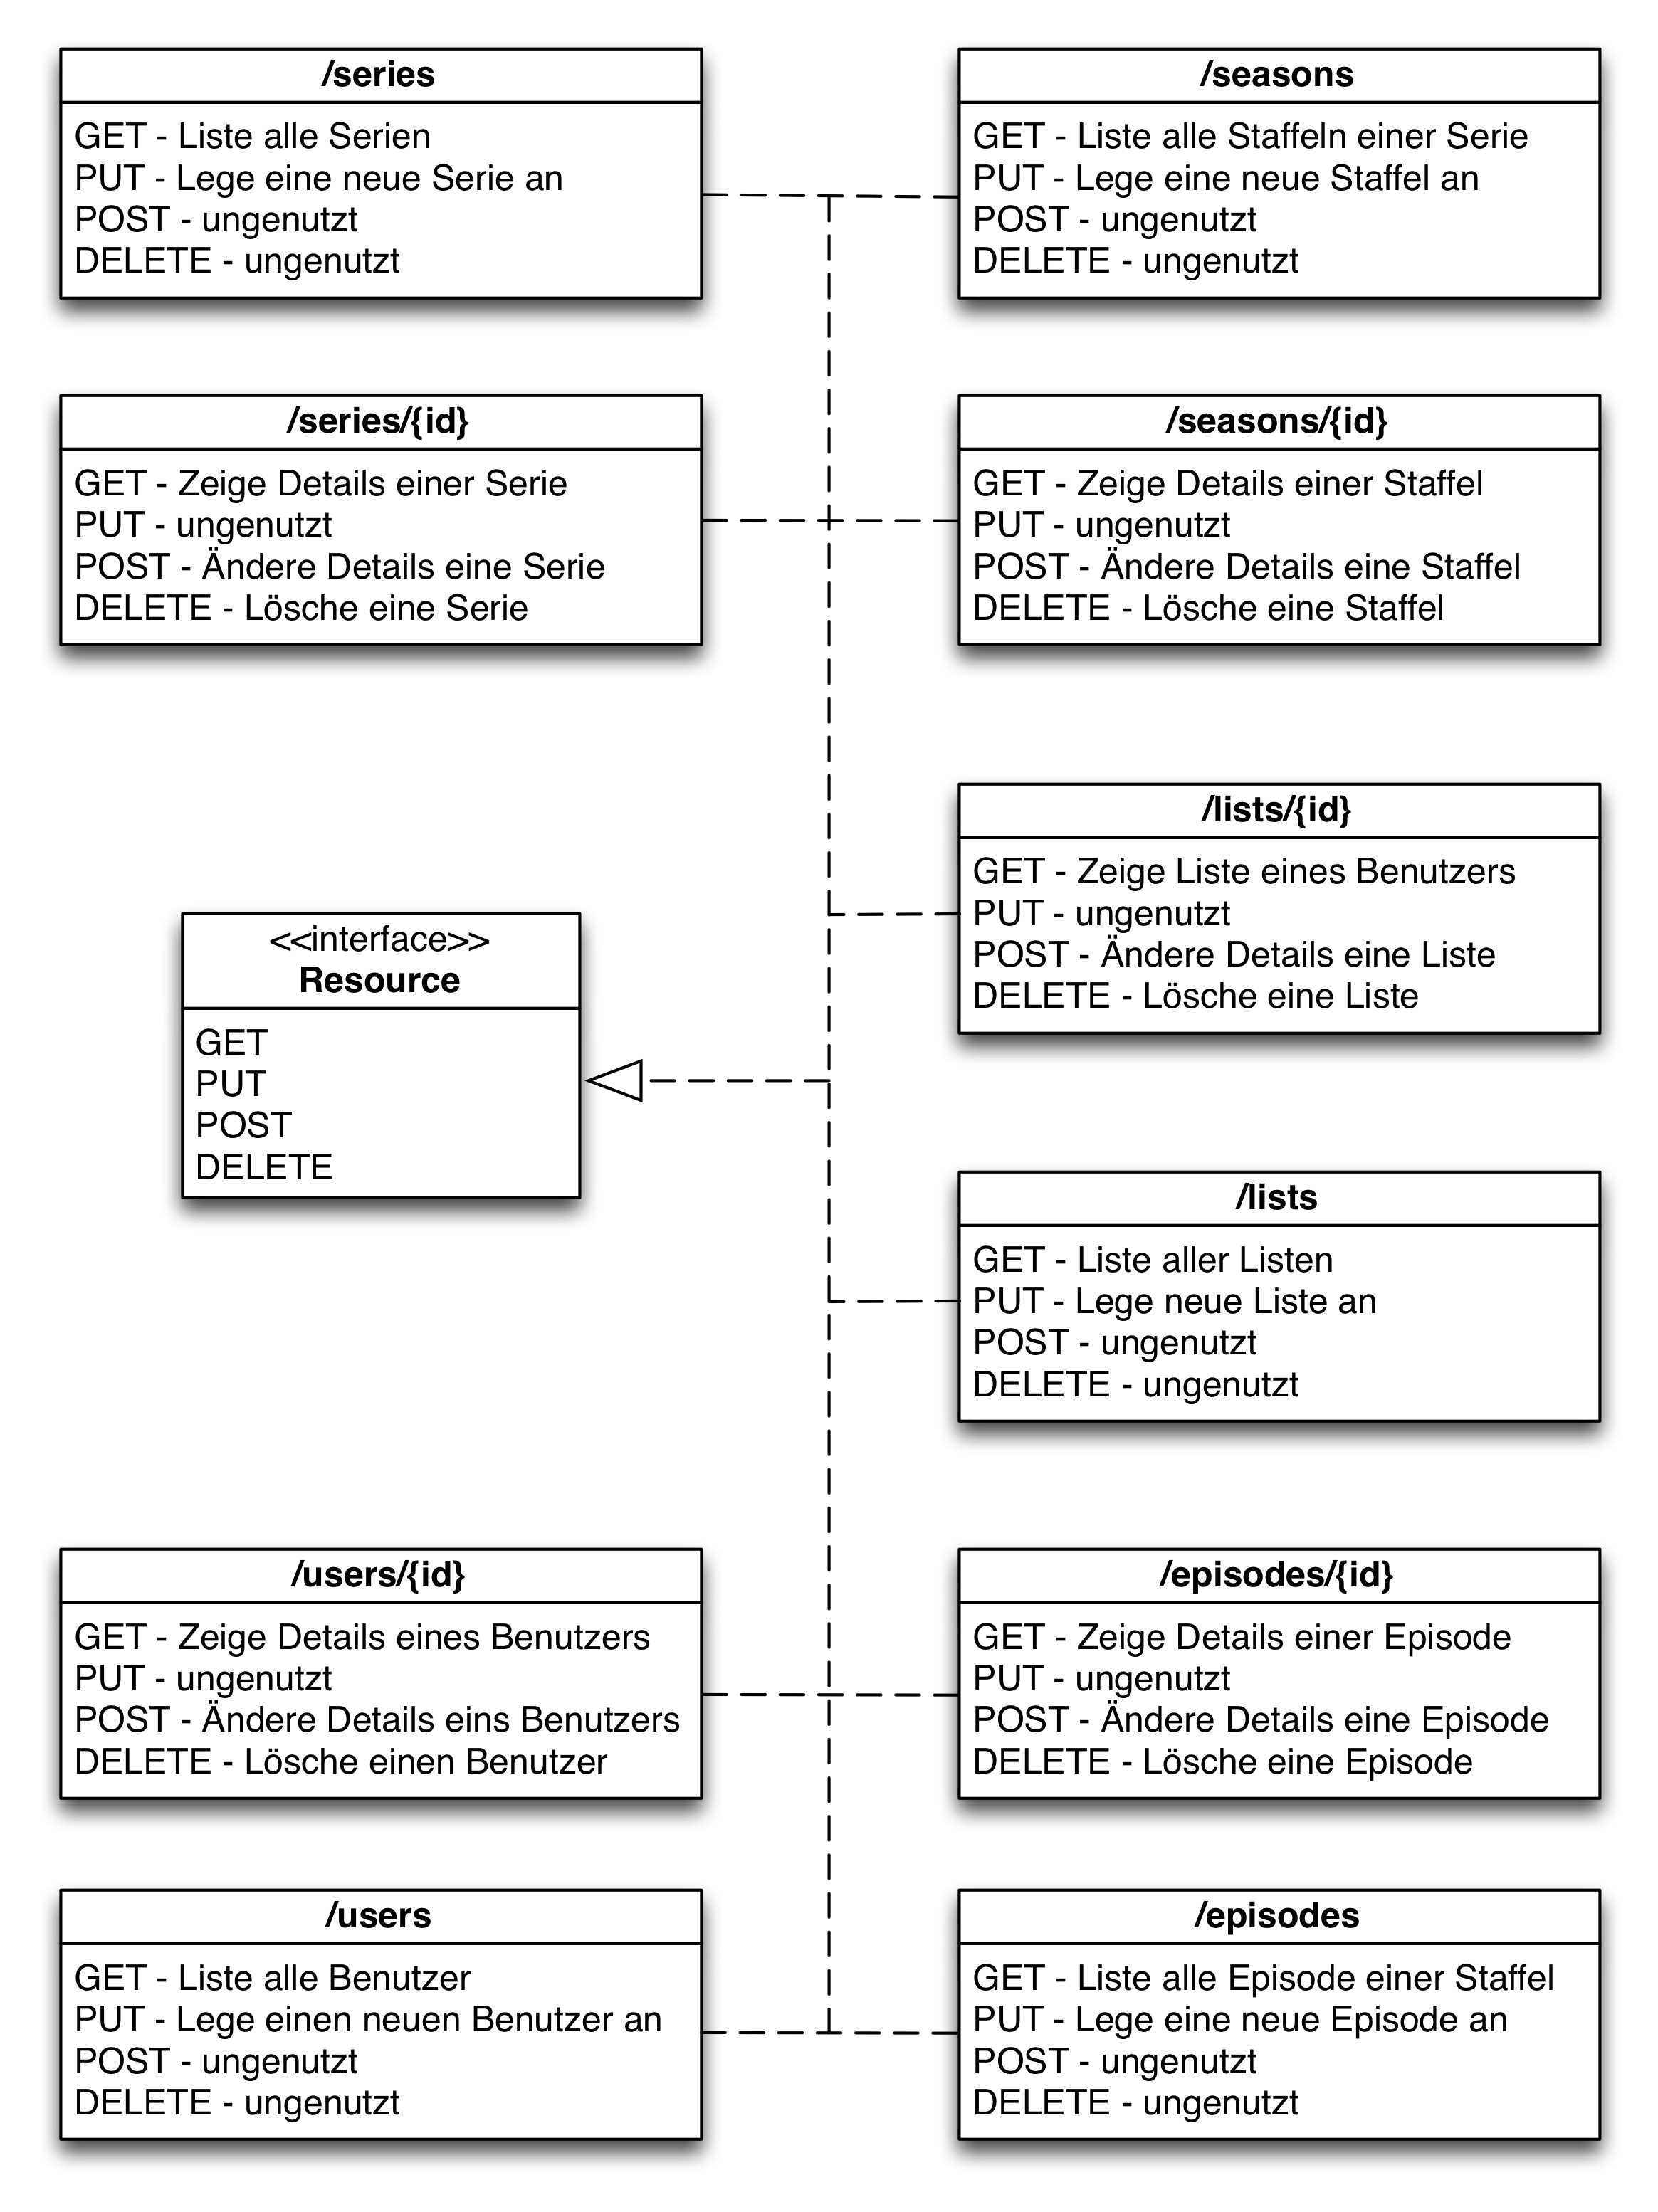
\includegraphics[width=1\textwidth]{images/bedeutunghttpmethoden.png}
\caption{Bedeutung der http Methoden}
\label{bedeutunghttpmethoden}
\end{figure}

\newpage


\subsection{RESTful Webservice}

\newpage

\subsection{Konzeption + XMPP Server einrichten}
Leafs (Topics) sollen für das Projekte definiert werden

Wer ist dabei Publisher und wer Subscriber?

Welche Daten sollen übetragen werden?

Entity
A JID-addressable Jabber entity (client, service, application, etc.).

Leaf Node
A type of node that contains published items only. It is NOT a container for other nodes.

Node
A virtual location to which information can be published and from which event notifications and/or payloads can be received (in other pubsub systems, this may be labelled a topic).

NodeID
The unique identifier for a node within the context of a pubsub service. The NodeID is either supplied by the node creator or generated by the pubsub service (if the node creator requests an Instant Node). The NodeID MAY have semantic meaning (e.g., in some systems or in pubsub profiles such as PEP the NodeID might be an XML namespace for the associated payload), but such meaning is OPTIONAL. If a document defines a given NodeID as unique within the realm of XMPP pubsub systems, it MUST specify the XML namespace of the associated payload.

Payload
The XML data that is contained within the <item/> element of a publication request or an event notification. A given payload is defined by an XML namespace and associated schema. A document that defines a payload format SHOULD specify whether the payload can be used only for a NodeID whose value is the same as the XML namespace, or whether the payload can be used for any NodeID. Such a document also SHOULD specify whether it is suggested that node at which such payloads are published are best configured as Singleton Nodes.

Publisher
Subscriber

Unterschiedliche Bedeutung von Node:
Service Discovery: Bereich der XMPP Entität, der den Umgang mit Anfragen und die Antwort bezüglich bestimmte Protokolle regelt.

<iq type='get'
    from='romeo@montague.net/orchard'
    to='mim.shakespeare.lit'
    id='info3'>
  <query xmlns='http://jabber.org/protocol/disco\#info' 
         node='http://jabber.org/protocol/commands'/>
</iq>
    


Publish Subscribe: Bestimmter Feed oder Channel, der in einem PubSub Service gehostet wird. Die Art des Channels wird durch den Payload charakterisiert.


<iq type='set'  
    from='hamlet@denmark.lit/blogbot'  
    to='pubsub.shakespeare.lit'  
    id='pub1'>  
  <pubsub xmlns='http://jabber.org/protocol/pubsub'>  
    <publish node='princely\_musings'>  
      <item>  
        <entry xmlns='http://www.w3.org/2005/Atom'>  
          <title>Soliloquy</title>  
          <summary>  
To be, or not to be: that is the question:  
Whether 'tis nobler in the mind to suffer  
The slings and arrows of outrageous fortune,  
Or to take arms against a sea of troubles,  
And by opposing end them?  
          </summary>  
          <link rel='alternate' type='text/html'  
                href='http://denmark.lit/2003/12/13/atom03'/>  
          <id>tag:denmark.lit,2003:entry-32397</id>  
          <published>2003-12-13T18:30:02Z</published>  
          <updated>2003-12-13T18:30:02Z</updated>  
        </entry>  
      </item>  
    </publish>  
  </pubsub>  
</iq>  


\newpage

\subsection{XMPP - Client}

Es soll ein XMPP Client entwickelt werden, dafür soll folgendes berücksichtigt werden:

Mittels der Anwendung soll es möglich sein Leafs zu abonnieren, Nachrichten zu empfangen und zu veröffentlichen.
Ermöglichen Sie die Übertragung von Nutzdaten (Beispielsweise Simplepayload)
Leafs und ggf. mögliche Eigenschaften der Leafs sollen angezeigt werden können (Service Discovery)
Service Discovery, disco: definiert in XEP-0030, 
2 wesentliche Methoden: disco\#items -> discover entities; disco\#info -> welche features werden von einer Entität unterstüzt

disco\#items: IQ-get an server gesendet, Replie liste der verbundenen EntitiesSimplepayload

\newpage

\subsection{Client - Entwicklung}

\newpage

\section{Projektreflektion}

\newpage

\listoffigures

\newpage 

\listoftables


\end{document}
